\newpage
\hypertarget{sec:breakpoints}{}
\section{Integrator Breakpoints}
\genHeader

When we introduced the integrator in \hyperlink{sec:app_integrator}{Part 6}, we showed you how it could be used to proceed through your transformation
incrementally. It shows the start point, possible rule candidates, and rule execution for every element. As you saw, this process
is great for reviewing a small transformation with only a few objects and rules as it doesn't take that long to run from start to finish. But what if you had a
transformation with 1000 objects, or 100 rules, and suspected there may be an error? As you can imagine, it would take a long time to find a specific trait.

Luckily, this visualized debugger is also able to implement a breakpoint model to pause the execution at any place! We extended our transformation in
the previous section with two rules able to handle partitions, so let's try implementing a breakpoint to pause the process before one of them is executed.

\begin{itemize}

\item[$\blacktriangleright$] You may have noticed when you ran the integrator for the first time that a new \texttt{BreakPointSet.xmi} file was created in
``instances/.'' Double-click this model, expand the tree, and create a new breakpoint (Fig.~\ref{eclipse:breakpointChild}).

\begin{figure}[htbp]
\begin{center}
  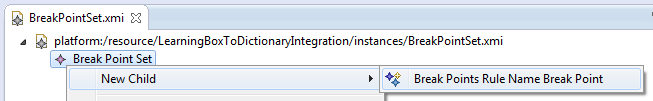
\includegraphics[width=\textwidth]{eclipse_breakpointChild}
  \caption{Create a new breakpoint instance}
  \label{eclipse:breakpointChild}
\end{center}
\end{figure}

\item[$\blacktriangleright$] Edit its \texttt{Rule Name} property below the editor to \texttt{AllOtherCardsRule} (Fig.~\ref{eclipse:bpProps}).\footnote{Be sure
there are no mistakes in the spelling} and save the file. This will pause the transformation before it applies the rule.

\begin{figure}[htbp]
\begin{center}
  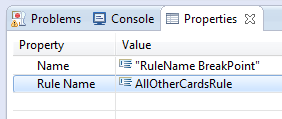
\includegraphics[width=0.5\textwidth]{eclipse_breakpointProperties}
  \caption{Completing the \texttt{Rule Name} breakpoint property}
  \label{eclipse:bpProps}
\end{center}
\end{figure}

\item[$\blacktriangleright$] Now start the integrator by right-clicking on \texttt{corr\_FWD}, then drag-and-drop the breakpoint model into
the main window. A small message should appear confirming that it is setting your breakpoint. 

\begin{figure}[htbp]
\begin{center}
  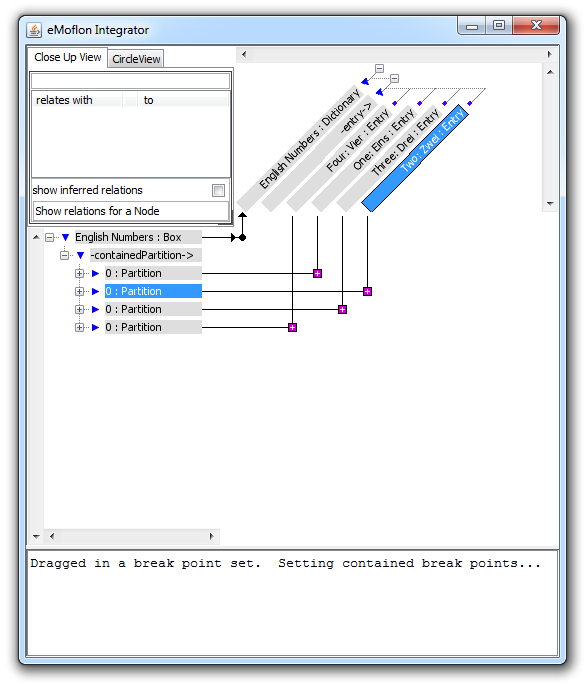
\includegraphics[width=0.8\textwidth]{eclipse_breakpointIntegrator}
  \caption{The integrator with an active breakpoint model}
  \label{eclipse:bpIntegrator}
\end{center}
\end{figure}

\item[$\blacktriangleright$] Finally, drag \texttt{protocol\_FWD} into the same window. You now have the ability to quickly skip between breakpoints
by pressing \texttt{alt\-+shift\-+ctrl\-+RIGHT} or backwards with \texttt{alt\-+shift\-+ctrl\-+LEFT}.

\end{itemize}

Please note that this particular breakpoint model will not stop the integrator if used on \texttt{corr\_BWD}. \texttt{AllOtherCardsRule} was only built to
operate on the source \texttt{Box} model, which means it will never be a valid candidate when transforming from \texttt{Dictionary}. Try experimenting with
\texttt{BoxToDictionaryRule} to see how this single breakpoint model works in both directions.
